\chapter{Lewisstructuren en de vorm van moleculen}\label{ch:g10:lewis-and-shape}

Een \omterm{def:g7:atoms-and-molecules:molecule}{molecuul} koolstofdioxide is recht; een watermolecuul is gebogen. Dat
ene verschil in vorm is een van de redenen waarom water, met \omterm{def:g7:atoms-and-molecules:molecule}{moleculen}
die lichter zijn dan die van koolstofdioxide, bij kamertemperatuur een
vloeistof is, terwijl koolstofdioxide een gas is. \omterm{def:g7:atoms-and-molecules:atom}{Atomen} in een \omterm{def:g7:atoms-and-molecules:molecule}{molecuul}
worden bij elkaar gehouden door gedeelde \omterm{def:g9:inside-the-atom:nucleus}{elektronen}, en de manier waarop
de \omterm{def:g9:inside-the-atom:nucleus}{elektronen} gedeeld worden, bepaalt de vorm. Dit hoofdstuk tekent de
gedeelde \omterm{def:g9:inside-the-atom:nucleus}{elektronen} en voorspelt daaruit de vorm.

\begin{recall}
De \omterm{def:g10:electron-shells:valence}{valentie-elektronen} zijn die van de buitenste \omterm{def:g10:electron-shells:configuration}{schil}; \omterm{def:g7:atoms-and-molecules:atom}{atomen} streven
naar de configuratie van een \omterm{def:g10:electron-shells:family}{edelgas}, acht \omterm{def:g9:inside-the-atom:nucleus}{elektronen} in de buitenste
\omterm{def:g10:electron-shells:configuration}{schil} (\omterm{def:g10:electron-shells:octet}{octetregel}) of twee voor waterstof (\omterm{def:g10:electron-shells:octet}{duetregel})
(\cref{ch:g10:electron-shells}). Molecuulmodellen tonen \omterm{def:g7:atoms-and-molecules:atom}{atomen} als
balletjes en bindingen als staafjes (\cref{ch:g7:atoms-and-molecules}).
\end{recall}

\section{De covalente binding}

\begin{definition}[Covalente binding]\label{def:g10:lewis-and-shape:covalent-bond}
Een \emph{covalente binding}\index{covalente binding} is een
elektronenpaar dat door twee \omterm{def:g7:atoms-and-molecules:atom}{atomen} gedeeld wordt; meestal levert elk
\omterm{def:g7:atoms-and-molecules:atom}{atoom} één \omterm{def:g9:inside-the-atom:nucleus}{elektron} van het paar. Beide \omterm{def:g7:atoms-and-molecules:atom}{atomen} tellen het gedeelde paar mee
in hun buitenste \omterm{def:g10:electron-shells:configuration}{schil}, waardoor ze allebei een duet of een octet kunnen
bereiken.
\end{definition}

\begin{definition}[Bindende en vrije elektronenparen]\label{def:g10:lewis-and-shape:lone-pair}
In een \omterm{def:g7:atoms-and-molecules:molecule}{molecuul} zijn de \omterm{def:g10:electron-shells:valence}{valentie-elektronen} van elk \omterm{def:g7:atoms-and-molecules:atom}{atoom} in paren
gegroepeerd. Een \emph{bindend elektronenpaar}\index{bindend elektronenpaar}
wordt door twee \omterm{def:g7:atoms-and-molecules:atom}{atomen} gedeeld en vormt een \omterm{def:g10:lewis-and-shape:covalent-bond}{covalente binding}; een
\emph{vrij elektronenpaar}\index{vrij elektronenpaar} hoort bij één \omterm{def:g7:atoms-and-molecules:atom}{atoom}
en doet niet mee aan een binding.
\end{definition}

\begin{proposition}[Hoeveel bindingen een atoom vormt]\label{prop:g10:lewis-and-shape:valence}
Een \omterm{def:g7:atoms-and-molecules:atom}{atoom} vormt evenveel \omterm{def:g10:lewis-and-shape:covalent-bond}{covalente bindingen} als het \omterm{def:g9:inside-the-atom:nucleus}{elektronen} tekortkomt
om zijn duet of octet te vervolledigen:
\begin{center}
\small
\begin{tabular}{lcccc}
\hline
\omterm{def:g7:atoms-and-molecules:atom}{atoom} & \omterm{def:g10:electron-shells:valence}{valentie-elektronen} & bindingen & vrije paren & voorbeeld \\
\hline
H & 1 & 1 & 0 & \ce{H2} \\
C & 4 & 4 & 0 & \ce{CH4} \\
N & 5 & 3 & 1 & \ce{NH3} \\
O & 6 & 2 & 2 & \ce{H2O} \\
Cl & 7 & 1 & 3 & \ce{HCl} \\
\hline
\hline
\end{tabular}
\end{center}
\end{proposition}

\section{Lewisstructuren}

\begin{definition}[Lewisstructuur]\label{def:g10:lewis-and-shape:lewis-structure}
De \emph{lewisstructuur}\index{lewisstructuur} van een \omterm{def:g7:atoms-and-molecules:molecule}{molecuul} toont de
\omterm{def:g7:atoms-and-molecules:atom}{atomen} met hun symbool, elk \omterm{def:g10:lewis-and-shape:lone-pair}{bindend elektronenpaar} als een streepje
tussen twee \omterm{def:g7:atoms-and-molecules:atom}{atomen} en elk \omterm{def:g10:lewis-and-shape:lone-pair}{vrij elektronenpaar} als twee puntjes naast zijn
\omterm{def:g7:atoms-and-molecules:atom}{atoom}.
\end{definition}

\begin{definition}[Dubbele en drievoudige bindingen]\label{def:g10:lewis-and-shape:multiple-bond}
Twee \omterm{def:g7:atoms-and-molecules:atom}{atomen} kunnen twee elektronenparen delen, een \emph{dubbele
binding}\index{dubbele binding}, getekend als twee streepjes, of drie
paren, een \emph{drievoudige binding}\index{drievoudige binding},
getekend als drie streepjes.
\end{definition}

\begin{method}[Een lewisstructuur tekenen]\label{met:g10:lewis-and-shape:draw}
\begin{enumerate}
  \item Tel de \omterm{def:g10:electron-shells:valence}{valentie-elektronen} van alle \omterm{def:g7:atoms-and-molecules:atom}{atomen} op, en deel door twee
        om het aantal paren te krijgen.
  \item Verbind de \omterm{def:g7:atoms-and-molecules:atom}{atomen} met enkele bindingen (waterstof, dat één binding
        vormt, zit altijd aan de buitenkant; koolstof staat meestal in het
        midden).
  \item Zet de overige paren als vrije paren neer, eerst op de buitenste
        \omterm{def:g7:atoms-and-molecules:atom}{atomen}, om hun octetten te vervolledigen.
  \item Heeft een \omterm{def:g7:atoms-and-molecules:atom}{atoom} nog geen octet, maak dan van een vrij paar van een
        buuratoom een tweede (of derde) gedeeld paar.
  \item Controleer: elke waterstof heeft 2 \omterm{def:g9:inside-the-atom:nucleus}{elektronen}, elk ander \omterm{def:g7:atoms-and-molecules:atom}{atoom} 8,
        en alle paren zijn gebruikt.
\end{enumerate}
\end{method}

\begin{example}[Koolstofdioxide]\label{ex:g10:lewis-and-shape:co2}
\ce{CO2}: $4 + 2 \times 6 = 16$ \omterm{def:g10:electron-shells:valence}{valentie-elektronen}, 8 paren. De enkele
bindingen \ce{O-C-O} gebruiken 2 paren; 6 vrije paren op de zuurstofatomen
maken die compleet, maar koolstof heeft dan maar 4 \omterm{def:g9:inside-the-atom:nucleus}{elektronen}. Door van
elk zuurstofatoom één vrij paar een gedeeld paar te maken, ontstaan twee
\omterm{def:g10:lewis-and-shape:multiple-bond}{dubbele bindingen}: nu heeft elk \omterm{def:g7:atoms-and-molecules:atom}{atoom} een octet.
\end{example}

\begin{omfigure}
\setchemfig{atom sep=2.0em}
\begin{tabular}{cccccc}
\chemfig{H-H} & \chemfig{H-\charge{0=\:,90=\:,270=\:}{Cl}} & \chemfig{H-\charge{90=\:,270=\:}{O}-H} &
\chemfig{H-\charge{90=\:}{N}(-[6]H)-H} & \chemfig{H-C(-[2]H)(-[6]H)-H} &
\chemfig{\charge{135=\:,225=\:}{O}=C=\charge{45=\:,315=\:}{O}} \\[4pt]
\small \ce{H2} & \small \ce{HCl} & \small \ce{H2O} & \small \ce{NH3} & \small \ce{CH4} & \small \ce{CO2} \\[10pt]
\chemfig{\charge{180=\:}{N}~\charge{0=\:}{N}} & \chemfig{\charge{135=\:,225=\:}{O}=\charge{45=\:,315=\:}{O}} &
\chemfig{C(-[3]H)(-[5]H)=C(-[1]H)-[7]H} & \chemfig{H-C~\charge{0=\:}{N}} &
\chemfig{H-C(-[6]H)=\charge{45=\:,315=\:}{O}} & \\[4pt]
\small \ce{N2} & \small \ce{O2} & \small \ce{C2H4} & \small \ce{HCN} & \small methanal \ce{CH2O} &
\end{tabular}

{\small \omterm{def:g10:lewis-and-shape:lewis-structure}{Lewisstructuren} van elf \omterm{def:g7:atoms-and-molecules:molecule}{moleculen}. Elk \omterm{def:g7:atoms-and-molecules:atom}{atoom} behalve waterstof is
omringd door vier paren (bindingen en vrije paren): een octet.}
\end{omfigure}

\section{De vorm van moleculen}

\begin{proposition}[Elektronenparen gaan zo ver mogelijk uit elkaar]\label{prop:g10:lewis-and-shape:shape}
Rond een centraal \omterm{def:g7:atoms-and-molecules:atom}{atoom} stoten de elektronengroepen --- elke enkele,
dubbele of \omterm{def:g10:lewis-and-shape:multiple-bond}{drievoudige binding}, en elk vrij paar --- elkaar af en gaan ze
zo ver mogelijk uit elkaar staan. Daaruit volgt de vorm van het \omterm{def:g7:atoms-and-molecules:molecule}{molecuul}:
\begin{center}
\small
\begin{tabular}{llll}
\hline
groepen rond het centrum & waarvan vrije paren & vorm & voorbeeld \\
\hline
2 & 0 & lineair, hoek \ang{180} & \ce{CO2}, \ce{HCN} \\
3 & 0 & vlakke driehoek, hoek \ang{120} & \ce{CH2O}, \ce{C2H4} \\
4 & 0 & tetraëder, hoek \ang{109.5} & \ce{CH4} \\
4 & 1 & piramide & \ce{NH3} \\
4 & 2 & gebogen & \ce{H2O} \\
\hline
\end{tabular}
\end{center}
\end{proposition}
\admitted

\begin{remark}[Waar dit vandaan komt]\label{rem:g10:lewis-and-shape:vsepr}
Deze regel is een model, en hij werkt opmerkelijk goed voor kleine
\omterm{def:g7:atoms-and-molecules:molecule}{moleculen}; hij wordt in het deel voor het eerste universiteitsjaar
preciezer gemaakt en deels verklaard. Vrije paren nemen iets meer ruimte
in dan bindende paren: de hoek in ammoniak (\ang{106.7}) en in water
(\ang{104.5}) is iets kleiner dan de \ang{109.5} van methaan.
\end{remark}

\begin{omfigure}
\begin{tikzpicture}[font=\small]
  % methane, tetrahedral, in perspective
  \begin{scope}
    \node[aC] (c) at (0,0) {};
    \node[aH, minimum size=3.6mm] (hb) at (0.3,-0.12) {};
    \node[aH] (h1) at (0,1.05) {};
    \node[aH] (h2) at (-1.0,-0.45) {};
    \node[aH] (h3) at (0.72,-0.5) {};
    \begin{scope}[on background layer]
      \foreach \h in {h1,h2,h3,hb} \draw[bond] (c.center) -- (\h.center);
    \end{scope}
    \node[aC] at (0,0) {};
    \node at (0,-1.35) {methaan: tetraëder};
    \node[font=\footnotesize] at (-0.55,0.55) {\ang{109.5}};
  \end{scope}
  % ammonia, pyramid
  \begin{scope}[xshift=4.2cm]
    \fill[omDef!25] (0,0.2) ellipse (0.18 and 0.45);
    \node[font=\scriptsize, omDef] at (0,1.0) {vrij paar};
    \node[aN] (n) at (0,0) {};
    \node[aH] (h1) at (-0.95,-0.5) {};
    \node[aH] (h2) at (0.7,-0.55) {};
    \node[aH, minimum size=3.6mm] (h3) at (0.25,-0.2) {};
    \begin{scope}[on background layer]
      \foreach \h in {h1,h2,h3} \draw[bond] (n.center) -- (\h.center);
    \end{scope}
    \node[aN] at (0,0) {};
    \node at (0,-1.35) {ammoniak: piramide};
  \end{scope}
  % water, bent
  \begin{scope}[xshift=8.4cm]
    \fill[omDef!25, rotate=25] (0,0.2) ellipse (0.16 and 0.42);
    \fill[omDef!25, rotate=-25] (0,0.2) ellipse (0.16 and 0.42);
    \node[aO] (o) at (0,0) {};
    \node[aH] (h1) at (-0.8,-0.58) {};
    \node[aH] (h2) at (0.8,-0.58) {};
    \begin{scope}[on background layer]
      \draw[bond] (o.center) -- (h1.center); \draw[bond] (o.center) -- (h2.center);
    \end{scope}
    \node[aO] at (0,0) {};
    \draw[black!60] (-0.32,-0.23) arc[start angle=216, end angle=324, radius=0.4];
    \node[font=\footnotesize] at (0,-0.65) {\ang{104.5}};
    \node at (0,-1.35) {water: gebogen};
  \end{scope}
  % carbon dioxide, linear
  \begin{scope}[xshift=12.0cm]
    \node[aO] (a) at (-0.8,0) {}; \node[aC] (c) at (0,0) {}; \node[aO] (b) at (0.8,0) {};
    \begin{scope}[on background layer]
      \foreach \d in {-1.6,1.6} {
        \draw[bond, line width=1.1pt] ([yshift=\d pt]a.center) -- ([yshift=\d pt]c.center);
        \draw[bond, line width=1.1pt] ([yshift=\d pt]c.center) -- ([yshift=\d pt]b.center);}
    \end{scope}
    \node at (0,-1.35) {koolstofdioxide: lineair};
  \end{scope}
\end{tikzpicture}

{\small Vormen van vier \omterm{def:g7:atoms-and-molecules:molecule}{moleculen} (vrije paren getekend als gearceerde
lobben).
% ledger: ang:H2O, ang:NH3
Methaan is een tetraëder, ammoniak een piramide, water gebogen,
koolstofdioxide recht.}
\end{omfigure}

\begin{omfigure}
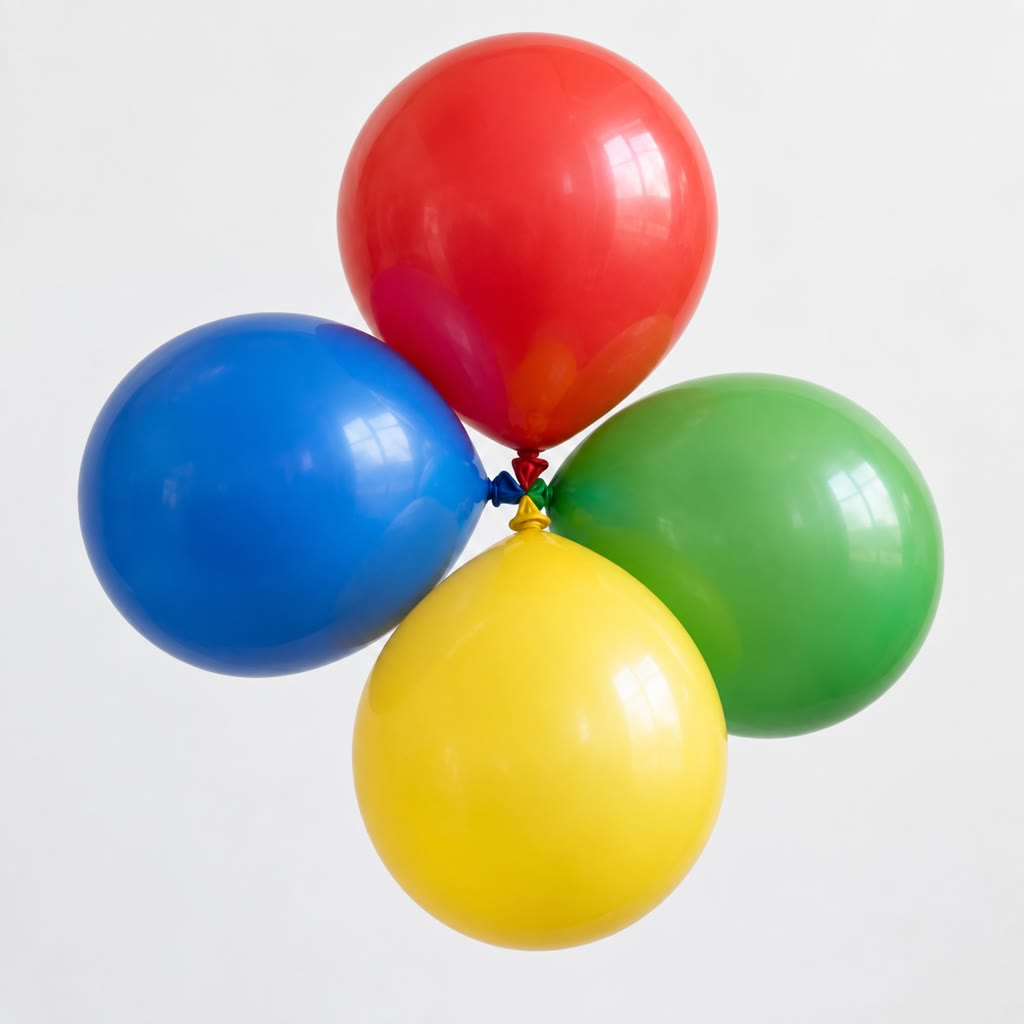
\includegraphics[width=0.38\linewidth]{images/book1/ai/g10-balloons-tetrahedron.jpg}

{\small Vier aan elkaar geknoopte ballonnen duwen elkaar zo ver mogelijk
weg; in de ruimte wijzen ze naar de hoekpunten van een tetraëder, net als
de vier elektronenparen rond een koolstofatoom.}
\end{omfigure}

\section{Moleculen in de ruimte tekenen}

\begin{notation}[Wiggen en streepjes]\label{not:g10:lewis-and-shape:wedge}
Om een \omterm{def:g7:atoms-and-molecules:molecule}{molecuul} in de ruimte op plat papier te tekenen, is een binding in
het vlak van het papier een gewone lijn, een binding die naar de lezer
toe wijst een volle wig, en een binding die van de lezer af wijst een
gestreepte wig. Methaan teken je dan zoals hieronder: twee bindingen in
het vlak, één naar de lezer toe en één van de lezer af.
\begin{center}
\chemfig{C(-[2]H)(-[4]H)(<[7]H)(<:[5]H)}
\end{center}
\end{notation}

\section{Oefeningen}

\begin{exercise}[$\star$]\label{exo:g10:lewis-and-shape:1}
Wat is een \omterm{def:g10:lewis-and-shape:covalent-bond}{covalente binding}? Wat is een \omterm{def:g10:lewis-and-shape:lone-pair}{vrij elektronenpaar}?
\end{exercise}

\begin{exercise}[$\star$]\label{exo:g10:lewis-and-shape:2}
Hoeveel \omterm{def:g10:lewis-and-shape:covalent-bond}{covalente bindingen} vormen waterstof, koolstof, stikstof en
zuurstof gewoonlijk? Leg uit met de octet- en de \omterm{def:g10:electron-shells:octet}{duetregel}.
\end{exercise}

\begin{exercise}[$\star$]\label{exo:g10:lewis-and-shape:3}
Teken de \omterm{def:g10:lewis-and-shape:lewis-structure}{lewisstructuur} van waterstofchloride, \ce{HCl}, en tel de
\omterm{def:g9:inside-the-atom:nucleus}{elektronen} rond chloor.
\end{exercise}

\begin{exercise}[$\star$]\label{exo:g10:lewis-and-shape:4}
Hoeveel \omterm{def:g10:electron-shells:valence}{valentie-elektronen} heeft het \omterm{def:g7:atoms-and-molecules:molecule}{molecuul} \ce{NH3} in totaal?
Hoeveel paren?
\end{exercise}

\begin{exercise}[$\star$]\label{exo:g10:lewis-and-shape:5}
Geef de vorm van \ce{CH4}, \ce{NH3}, \ce{H2O} en \ce{CO2}.
\end{exercise}

\begin{exercise}[$\star\star$]\label{exo:g10:lewis-and-shape:6}
Teken de \omterm{def:g10:lewis-and-shape:lewis-structure}{lewisstructuur} van waterstofsulfide, \ce{H2S} (zwavel staat in
de groep van zuurstof), en voorspel de vorm.
\end{exercise}

\begin{exercise}[$\star\star$]\label{exo:g10:lewis-and-shape:7}
Teken de \omterm{def:g10:lewis-and-shape:lewis-structure}{lewisstructuur} van stikstof, \ce{N2}, en volg de methode stap
voor stap.
\end{exercise}

\begin{exercise}[$\star\star$]\label{exo:g10:lewis-and-shape:8}
Teken de \omterm{def:g10:lewis-and-shape:lewis-structure}{lewisstructuur} van methanol, \ce{CH3OH}, en geef de vorm rond
het koolstofatoom en rond het zuurstofatoom.
\end{exercise}

\begin{exercise}[$\star\star$]\label{exo:g10:lewis-and-shape:9}
Waarom is \ce{CO2} lineair en \ce{H2O} gebogen, hoewel ze allebei een
centraal \omterm{def:g7:atoms-and-molecules:atom}{atoom} hebben dat aan twee andere vastzit?
\end{exercise}

\begin{exercise}[$\star\star$]\label{exo:g10:lewis-and-shape:10}
Teken de \omterm{def:g10:lewis-and-shape:lewis-structure}{lewisstructuur} van etheen, \ce{C2H4}, en geef de vorm rond elk
koolstofatoom.
\end{exercise}

\begin{exercise}[$\star\star$]\label{exo:g10:lewis-and-shape:11}
Teken de \omterm{def:g10:lewis-and-shape:lewis-structure}{lewisstructuur} van tetrachloormethaan, \ce{CCl4}, en voorspel
de vorm.
\end{exercise}

\begin{exercise}[$\star\star\star$]\label{exo:g10:lewis-and-shape:12}
Twee \omterm{def:g7:atoms-and-molecules:molecule}{moleculen} hebben de formule \ce{C2H6O}. Teken voor elk een
\omterm{def:g10:lewis-and-shape:lewis-structure}{lewisstructuur} (het ene heeft een O--H-binding, het andere een
C--O--C-keten).
\end{exercise}

\begin{exercise}[$\star\star\star$]\label{exo:g10:lewis-and-shape:13}
Leg met vrije paren uit waarom de hoek in ammoniak (\ang{106.7}) kleiner
is dan in methaan (\ang{109.5}), en in water (\ang{104.5}) nog kleiner.
\end{exercise}

\begin{exercise}[$\star\star\star$]\label{exo:g10:lewis-and-shape:14}
Teken de \omterm{def:g10:lewis-and-shape:lewis-structure}{lewisstructuur} van waterstofcyanide, \ce{HCN}, en van methanal,
\ce{CH2O}, en geef hun vorm.
\end{exercise}

\begin{exercise}[$\star\star\star$]\label{exo:g10:lewis-and-shape:15}
Ozon, \ce{O3}, is een keten van drie zuurstofatomen. Tel zijn
valentieparen en teken een \omterm{def:g10:lewis-and-shape:lewis-structure}{lewisstructuur} waarin elk zuurstofatoom een
octet heeft (één \omterm{def:g10:lewis-and-shape:multiple-bond}{dubbele binding}, één enkele binding). Voorspel of het
\omterm{def:g7:atoms-and-molecules:molecule}{molecuul} lineair of gebogen is.
\end{exercise}

\section{Probleem: Een molecuul in een kubus}

\begin{problem}[{Weekendprobleem --- de koolstofballetjes van een
molecuulbouwdoos ontwerpen: onder welke hoek moeten de gaatjes geboord
worden?}]
\label{pb:g10:lewis-and-shape:1}
% ledger: ang:H2O, ang:NH3
Een bedrijf maakt molecuulbouwdozen. De zwarte koolstofballetjes moeten
vier gaatjes hebben, zodat methaan, ethaan en de andere
koolstofmoleculen de juiste vorm krijgen. De ingenieur gebruikt een
truc: een regelmatige tetraëder past in een kubus, met zijn vier
hoekpunten op vier hoekpunten van de kubus, waarvan er geen twee op
dezelfde ribbe liggen.

\medskip
\noindent\textbf{Deel I --- \omterm{def:g10:lewis-and-shape:lewis-structure}{Lewisstructuren}.}
\begin{enumerate}
  \item Teken de \omterm{def:g10:lewis-and-shape:lewis-structure}{lewisstructuren} van methaan \ce{CH4}, ammoniak \ce{NH3}
        en water \ce{H2O}.
  \item Hoeveel elektronengroepen omringen het centrale \omterm{def:g7:atoms-and-molecules:atom}{atoom} in elk?
  \item Hoeveel daarvan zijn vrije paren?
  \item Waarom heeft een koolstofballetje vier gaatjes nodig, en een
        zuurstofballetje (voor water) maar twee?
  \item Een model van ethaan, \ce{C2H6}, gebruikt twee
        koolstofballetjes. Teken de \omterm{def:g10:lewis-and-shape:lewis-structure}{lewisstructuur}. Hoeveel staafjes
        verbinden de twee koolstofballetjes, en hoeveel
        waterstofballetjes zijn er nodig?
\end{enumerate}

\medskip
\noindent\textbf{Deel II --- Vormen.}
\begin{enumerate}[resume]
  \item Geef de vorm van elk van de drie \omterm{def:g7:atoms-and-molecules:molecule}{moleculen}.
  \item De gemeten hoeken zijn \ang{106.7} in ammoniak en \ang{104.5} in
        water. Leg uit waarom ze kleiner zijn dan de hoek van methaan.
  \item Waarom kan het zuurstofballetje voor water niet gewoon een
        koolstofballetje zijn waarvan twee gaatjes leeg blijven, als de
        bouwdoos de echte hoek moet laten zien?
  \item In koolstofdioxide vormt het koolstofatoom twee \omterm{def:g10:lewis-and-shape:multiple-bond}{dubbele
        bindingen}. Welke hoek moet ze in een model scheiden?
\end{enumerate}

\medskip
\noindent\textbf{Deel III --- De kubus.}
Neem een kubus met ribbe $a$. Het koolstofatoom zit in het middelpunt; de
vier waterstofatomen zitten op vier hoekpunten van de kubus, waarvan er
geen twee op dezelfde ribbe liggen.
\begin{enumerate}[resume]
  \item Laat zien dat elk tweetal van deze waterstofatomen op de twee
        uiteinden van een diagonaal van een zijvlak van de kubus ligt.
        Bereken met de stelling van Pythagoras hun afstand, uitgedrukt in
        $a$.
  \item De diagonaal van de hele kubus (van een hoekpunt naar het
        tegenoverliggende hoekpunt) heeft lengte $a\sqrt{3}$. Leid daaruit
        de afstand van het koolstofatoom tot een waterstofatoom af.
  \item Neem $a = \qty{1}{cm}$ in een model: geef beide afstanden in
        centimeter, op twee decimalen.
  \item Waarom zijn de vier C--H-afstanden gelijk?
\end{enumerate}

\medskip
\noindent\textbf{Deel IV --- De hoek.}
Het koolstofatoom C en twee waterstofatomen H$_1$, H$_2$ vormen een
gelijkbenige driehoek. Zij M het midden van H$_1$H$_2$.
\begin{enumerate}[resume]
  \item Leg uit waarom driehoek C\,M\,H$_1$ een rechte hoek heeft bij M.
  \item Bereken in deze rechthoekige driehoek de sinus van hoek
        $\widehat{\text{M\,C\,H}_1}$, de helft van hoek H--C--H.
  \item Leid daaruit de halve hoek af, en daarna hoek H--C--H, op één
        decimaal.
  \item Vergelijk met de hoek uit de tabel van dit hoofdstuk.
  \item Geef de hoek waaronder de gaatjes van een koolstofballetje
        geboord moeten worden.
\end{enumerate}
\end{problem}
